%%%%%%%%%%%%%%%%%%%% author.tex %%%%%%%%%%%%%%%%%%%%%%%%%%%%%%%%%%%
%
% sample root file for your "contribution" to a contributed volume
%
% Use this file as a template for your own input.
%
%%%%%%%%%%%%%%%% Springer %%%%%%%%%%%%%%%%%%%%%%%%%%%%%%%%%%


% RECOMMENDED %%%%%%%%%%%%%%%%%%%%%%%%%%%%%%%%%%%%%%%%%%%%%%%%%%%
\documentclass[graybox]{svmult}

% choose options for [] as required from the list
% in the Reference Guide

\usepackage{type1cm}        % activate if the above 3 fonts are
                            % not available on your system
%
\usepackage{makeidx}         % allows index generation
\usepackage{graphicx}        % standard LaTeX graphics tool
                             % when including figure files
\usepackage{multicol}        % used for the two-column index
\usepackage[bottom]{footmisc}% places footnotes at page bottom
\usepackage{multirow}


\usepackage{newtxtext}       % 
\usepackage{newtxmath}       % selects Times Roman as basic font

% see the list of further useful packages
% in the Reference Guide

\makeindex             % used for the subject index
                       % please use the style svind.ist with
                       % your makeindex program

%%%%%%%%%%%%%%%%%%%%%%%%%%%%%%%%%%%%%%%%%%%%%%%%%%%%%%%%%%%%%%%%%%%%%%%%%%%%%%%%%%%%%%%%%

\begin{document}

\title*{Bento Packaging Activity Recognition with Convolutional LSTM using Autocorrelation Function and Majority Vote}
\titlerunning{Bento Packaging Activity Recognition with Convolutional LSTM}
% Use \titlerunning{Short Title} for an abbreviated version of
% your contribution title if the original one is too long
\author{Atsuhiro Fujii, Kazuki Yoshida, Kiichi Shirai, Kazuya Murao}
% Use \authorrunning{Short Title} for an abbreviated version of
% your contribution title if the original one is too long
\institute{Asuhiro Fujii, \at Graduate School of Information Science and Engineering, Ritsumeikan University, 1-1-1 Nojihigashi, Kusatsu, Shiga 525-8577, Japan %\email{atsuhiro.fujii@iis.ise.ritsumei.ac.jp}
\and Kazuki Yoshida \at Graduate School of Information Science and Engineering, Ritsumeikan University, 1-1-1 Nojihigashi, Kusatsu, Shiga 525-8577, Japan %\email{kazuki.yoshida@iis.ise.ritsumei.ac.jp}
\and Kiichi Shirai \at Graduate School of Information Science and Engineering, Ritsumeikan University, 1-1-1 Nojihigashi, Kusatsu, Shiga 525-8577, Japan %\email{kiichi.shirai@iis.ise.ritsumei.ac.jp}
\and Kazuya Murao \at Graduate School of Information Science and Engineering, Ritsumeikan University, 1-1-1 Nojihigashi, Kusatsu, Shiga 525-8577, Japan \email{murao@cs.ritsumei.ac.jp}}
%
% Use the package "url.sty" to avoid
% problems with special characters
% used in your e-mail or web address
%
\maketitle

\abstract{This paper reports Bento Packaging Activity Recognition Challenge by team ``RitsBen'' held in the International Conference on Activity and Behavior Computing (ABC 2021). Our approach leverages autocorrelation function to extract repetitive behaviors from the dataset. We then use a model that implements convolution layer and LSTM, to recognize the activities. The loss is calculated using BCEWithLogitsLoss for each body part, and then the final decision is made by majority vote using sigmoid predictions output from all body parts.}

% 1
\section{Introduction}
\label{sec:introduction}
This paper reports the solution of our team ``RitsBen'' to Bento Packaging Activity Recognition Challenge held at International Conference on Activity and Behavior Computing (ABC2021). 
% 本論文は、International Conference on Activity and Behavior Computing (ABC2021)で開催されたBento Packaging Activity Recognition Challengeに対する我々のチーム ``RitsBen''のソリューションを報告するものである。
The goal of Bento Packaging Activity Recognition Challenge is to distinguish activities taking place during each segment based on the motion data collected with motion capture sensors while performing Bento-box packaging tasks. Activity recognition is the process of automatically inferring what a user is doing based on sensor observations. Since activity recognition can enrich our lives by understanding the characteristics of human activity, there have been a lot of research on human activity recognition (HAR). 
% ABC2021の目標は、弁当箱詰め作業を行う際にモーションキャプチャーセンサーで収集したモーションデータに基づいて、各セグメントで行われているアクティビティを識別することです。アクティビティ認識とは、センサーの観測結果に基づいて、ユーザーが何をしているかを自動的に推論するプロセスである。活動認識は人間の行動の特徴を把握することで我々の生活を豊かにすることができるため、人間の活動認識(HAR)に関する研究が盛んに行われている。

Lara et al.\cite{lara2012survey} surveyed  the state of the art in HAR based on wearable sensors.
% Lara et al.はウェアラブルセンサーを利用したHARの現状を調査した。
Khan et al.\cite{khan2010triaxial} proposed an accelerometer-based HAR method.
% Khan et al.は加速度センサを用いたHAR手法を提案した。
Bayat et al.\cite{bayat2014study} proposed a recognition system in which a new digital low-pass filter is designed.
% Bayat et al.は新しいデジタルローパスフィルタを設計した認識システムを提案した。
Anguita et al.\cite{anguita2012human} conducted a comparative study on HAR using inertial sensors in a smartphone.
% Anguita et al.は、スマートフォンの慣性センサーを用いたHARの比較研究を行った。
Attal et al.\cite{attal2015physical} presents a review of different classification techniques in HAR based on wearable inertial sensors.
% Attal et al.はHARに使用される分類技術の評価を行なった。
% 
In recent years, methods that use neural networks to improve the accuracy of activity recognition have also been actively researched.
% また、近年では活動認識の精度を高めるためにニューラルネットワークを用いる手法が盛んに研究されています。
Yang et al.\cite{yang2015deep} propose a systematic feature learning method based on deep convolutional neural networks (CNN) for HAR problem.
% Yang et al.は深層畳み込みニューラルネットワークを用いた系統的な特徴学習手法を提案した
Chen et al.\cite{chen2015deep} proposed a deep learning approach to HAR based on single accelerometer. 
%Chenらは、3軸加速度センサのデータを用いて人間の活動を認識するために、LSTMベースの特徴抽出アプローチを提案しました。
Tsokov et al.\cite{tsokov2021evolutionary} proposed an evolutionary based approach for optimizing the architecture of one dimensional CNNs for HAR.
% Tsokov et al.はHARのための1次元CNNのアーキテクチャを最適化するための進化論的アプローチを提案した。
Dang et al.\cite{dang2020sensor} introduced a classification of HAR methodologies, and shows advantages and weaknesses for methods in each category.
% Danga et al.は近年のHAR手法の分類を紹介し、各分類に属する手法の利点と弱点を示した。

%The activity dataset prepared for this challenge includes the training dataset and the test dataset. In the training dataset, data of three subjects have been provided along with all activity labels. In the test dataset, unlabeled data of the other subject has been given.
% 本チャレンジで用意された活動データセットにはトレーニングデータセットとテストデータセットがある。トレーニングデータセットでは3人の被験者のデータとすべてのアクティビティのラベルを提供しています。テストデータセットでは、残りの被験者のラベルなしのデータが与えられています。
In this paper we construct a network with convolutional layer and LSTM layer to recognize the activities and detected repetition using autocorrelation function. The outputs of the model are sigmoid values, the number of the outputs is as much as the number of sensors. The final output is a majority vote on those sigmoid values.
%本論文では,アクティビティを認識するために,畳み込み層とLSTM層を用いたネットワークを構築と自己相関関数を用いて繰り返しを検出した.モデルの出力はシグモイド値で、出力の数はセンサーの数と同数です。
%最終出力はそれらのシグモイド値を多数決する
%



% 2
\section{Challenge}
\label{sec:challenge}
%このチャレンジでは,各チームが弁当箱へ詰め込みに関する活動の認識精度を競い合う.ここでは,チャレンジの目的,データセットの内容,評価基準を述べる.
In this challenge, each team competes in the recognition accuracy of activities related to Bento-box packaging. This section introduces the challenge goal, the contents of dataset, and the evaluation criteria.


\subsection{Challenge Goal}
%Bento Packaging Activity Recognition Challengeの目標は,モーションキャプチャーデータに基づいて,10種類の弁当詰め込み作業を認識することである.
The goal of the Bento Packaging Activity Recognition Challenge is to recognize the Bento-box packaging activities based on motion capture data.
%学習データセットは3人の被験者から採取したデータで,すべての行動のラベルが含まれている.テストデータセットにはもう1人の被験者から採取したデータで,行動のラベルは付けられていない.参加者は自身が作成したモデルを使用して,テストデータを使って予測した行動を提出する必要がある.
The training dataset contains data about all activity labels collected from three subjects. The test dataset contains data that is not labeled collected from the other subject. The challenge participants must submit their predicted Bento-box packaging activities on the test dataset using their models.

\subsection{Dataset}
\label{subsec:dataset}
This section introduces the dataset used for this challenge. For more details, please refer to the article\cite{ex1}.

\subsubsection{Sensors and subjects}
%Motion Analysis Company社製のモーションキャプチャーシステムを使用して,29点のマーカーを装着した4人の被験者(全員男性)からデータを採取した.被験者は3種類の食材を5種類の弁当箱への詰め込みシナリオに従って行った.各シナリオは外向きと内向きの2パターンで5回ずつ行った.合計で,4人の被験者×5種類のシナリオ×2パターン×5回=200回の試行を行った.
The data collected from four subjects (all males) who attached one motion capture system with 29 markers released by Motion Analysis Company\footnote{https://motionanalysis.com}. The subjects packed three types of food according to the five different bento-box packaging scenarios. The subjects performed in two patterns of outward and inward, and five times each scenario. In total, 4 subjects $\times$ 5 scenarios $\times$ 2 patterns $\times$ 5 trials = 200 of data were collected.
%本来,学習データセットには3人の被験者分の150件のデータが含まれてなければならない.しかし,被験者1の行動ラベル6では5回目の試行が無く,被験者2の行動ラベル6と9には6回目の試行が含まれていた.したがって,学習データセットで配布されたデータは151件であった.
Originally, the training dataset should be contained 150 trials for three subjects. However, activity 6 of subject 1 did not contain the fifth trial and the activity 6 and 9 of subject 2 contained the sixth trial. Therefore, the total number of training data was 151.

\subsubsection{Data structure}
%学習データには4人の被験者のうち3人の被験者(被験者1,2,3)のデータが含まれている.テストデータには4人目の被験者(被験者4)のデータが含まれている.
Training data contains data from three subjects (subjects 1, 2, 3) out of the four subjects and test data contains the data from the fourth subject (subject 4).
%表\ref{tab:activity}に10種類の行動名と動作方向のパターン,および行動ラベル番号の一覧を示す.5種類の行動タイプと2種類の動作方向パターンがあり,合計で10種類(5 \times 2 = 10)となっている.
Table \ref{tab:activity} shows a list of 10 different activity names, movement direction patterns, and activity labels; there are 5 different activity types, and 2 movement direction patterns, for a total of 10 types ($5 \times 2 = 10$).
%被験者,行動ラベル,試行回数ごとにセグメントが分割保存されている.例えば,{\tt [subject\verb|_|1\verb|_|activity\verb|_|1\verb|_|repeat\verb|_|1]}ならば,このセグメントで被験者1が行動ラベル1の1回目の試行をしていることを意味する.
The segment is stored and divided by subject, activity label, and trials. For example, {\tt [subject\verb|_|1\verb|_|activity\verb|_|1\verb|_|repeat\verb|_|1]} contain the data of subject 1 having performed the first trial of activity whose label number is 1.
%1つのファイルには装着したマーカー29点それぞれから計測した3軸(X,Y,Z)データ,被験者番号,行動ラベル番号の合計89種類のデータが保存されている.1ファイルの計測時間はそれぞれ50秒から70秒である.
Each file contains 89 types of data: 3-axis (X, Y, Z) data measured from each of 29 markers, subject number, and activity label. The measurement time for each file ranges from 50 to 70 s.
%なお,モーションキャプチャーセンサの設定が複雑であったため,計測データの欠損や行動ラベルの誤りが含まれている場合がある.
Note that due to the complicated setup of the motion capture sensor, missing measurement data and incorrect activity labels may be included.


\begin{table}[h]
    \centering
    \caption{A list of 10 different activity names, movement direction patterns, and activity labels.}
    \begin{tabular}{c|c|c}\hline\hline
    Activity name & Movement direction pattern & Activity label \\ \hline
    \multirow{2}{*}{Normal} & Inward & 1 \\ \cline{2-3}
    & Outward & 2 \\ \hline
    \multirow{2}{*}{Forgot to put ingredients} & Inward & 3 \\ \cline{2-3}
    & Outward & 4 \\ \hline
    \multirow{2}{*}{Failed to put ingredients} & Inward & 5 \\ \cline{2-3}
    & Outward & 6 \\ \hline
    \multirow{2}{*}{Turn over bento-box} & Inward & 7 \\ \cline{2-3}
    & Outward & 8 \\ \hline
    \multirow{2}{*}{Fix/rearranging ingredients} & Inward & 9 \\ \cline{2-3}
    & Outward & 10 \\ \hline
    \end{tabular}
    \label{tab:activity}
\end{table}

\subsubsection{Statistics}
%表\ref{tab:stats}に被験者ごとの認識するクラス数(本チャレンジでは10クラス),セグメント数,各行動ラベルにおける試行回数の最大値,最小値,平均値,セグメントの長さの最大値,平均値,最小値を示す.
Table \ref{tab:stats} shows the number of recognized classes (10 classes in this challenge), the number of segments for each subject, the number of trials for each activity, and the maximum, mean, and minimum length of the segments.

\begin{table}[h]
    \centering
    \caption{Statistics of the dataset.}
    \begin{tabular}{c|c|c|c|c|c|c|c}\hline\hline
    Subject & Activity label& \# of recognized classes & \# of segments & \# of trials & \multicolumn{3}{c}{Length} \\
    &&&&&max&mean&min\\\hline
    \multirow{10}{*}{1} & 1 & \multirow{10}{*}{10} & \multirow{10}{*}{49} & 5 & 5701 & 5311 & 5516\\
    & 2 & & & 5 & 6325 & 5120 & 5860\\
    & 3 & & & 5 & 6448 & 5956 & 6214\\
    & 4 & & & 5 & 6665 & 6257 & 6446\\
    & 5 & & & 5 & 6467 & 5955 & 6310\\
    & 6 & & & 4 & 5771 & 5427 & 5525\\ 
    & 7 & & & 5 & 5725 & 5323 & 5567\\ 
    & 8 & & & 5 & 6653 & 6307 & 6395\\ 
    & 9 & & & 5 & 6828 & 6252 & 6530\\
    & 10 & & & 5 &6962 & 6269 & 6525\\ \hline
    \multirow{10}{*}{2} & 1 & \multirow{10}{*}{10} & \multirow{10}{*}{52} & 5 & 7660 & 6626 & 7037\\
    & 2 & & & 5 & 6788 & 6493 & 6667\\
    & 3 & & & 5 & 6827 & 6390 & 6610\\ 
    & 4 & & & 5 & 6933 & 6295 & 6564\\
    & 5 & & & 5 & 6690 & 6470 & 6608\\
    & 6 & & & 6 & 8441 & 7660 & 7996\\
    & 7 & & & 5 & 7719 & 7392 & 7511\\
    & 8 & & & 5 & 7870 & 7386 & 7667\\ 
    & 9 & & & 6 & 7434 & 1663 & 6343\\
    & 10 & & & 5 &7420 & 6651 & 6343\\ \hline
    \multirow{10}{*}{3} & 1 & \multirow{10}{*}{10} & \multirow{10}{*}{50} & 5 & 6337 & 5972 & 6149\\
    & 2 & & & 5 & 6326 & 5724 & 5915\\
    & 3 & & & 5 & 5995 & 5582 & 5801\\
    & 4 & & & 5 & 5930 & 5596 & 5768\\
    & 5 & & & 5 & 5953 & 5523 & 5778\\
    & 6 & & & 5 & 6190 & 5402 & 5769\\
    & 7 & & & 5 & 6017 & 5408 & 5737\\ 
    & 8 & & & 5 & 5718 & 5223 & 5459\\
    & 9 & & & 5 & 5860 & 5357 & 5620\\
    & 10 & & & 5 &5714 & 5351 & 5579\\ \hline
    4 & Unknown & 10 & 48 & Unknown & 5947 & 5024 & 5481\\ \hline
    \end{tabular}
    \label{tab:stats}
\end{table}

\subsection{Evaluation criteria}
%投稿結果は,10種類の行動の精度で評価される.精度は予測したラベルで正しかった数を予測したデータ数で割った値で求められる.
Submissions from the participants will be evaluated by the accuracy of activity classification. The accuracy is given by $accuracy = \frac{P\cap G}{P\cup G}$; the number of correct labels predicted (logical product of prediction set $P$ and groundtruth set $G$) divided by the number of total true and predicted labels (logical sum of $P$ and $G$).

% 3
\section{Method}
\label{sec:method}
This section describes the preprocessing to obtain the features from the raw data, the structure of the model, the loss function and the optimizer, and the process of obtaining the activity labels from the predictions obtained by the one-hot vector. Note that our method does not use motion capture data.


\subsection{Preprocessing}
Figure \ref{fig:preprocess} shows the flow of preprocessing. The details of each process are described below.

\begin{figure}[h]
    \centering
    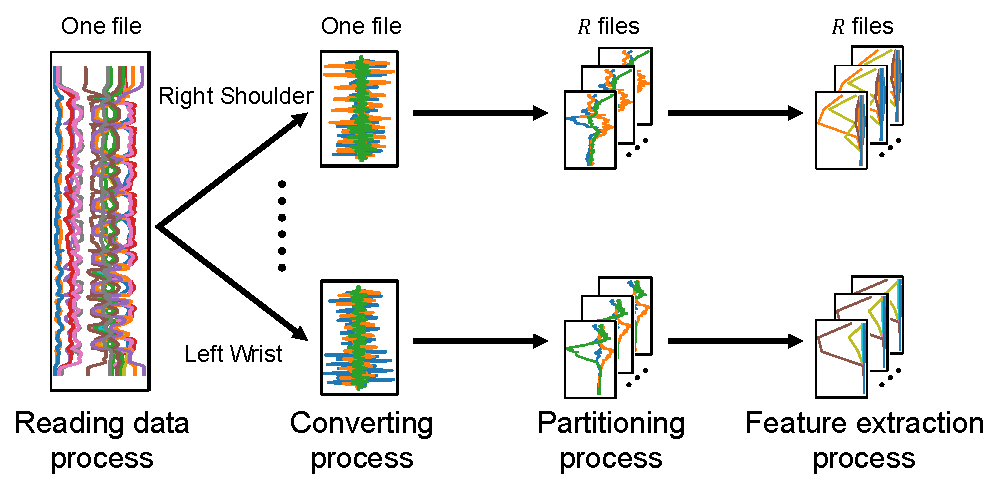
\includegraphics[width=0.7\linewidth]{figures/preprocess.eps}
    \caption{Details of preprocessing. The first process is the raw data as it is provided. In the second process, the raw data is converted to velocity data. The partitioning process identifies and separates repetitive parts from the velocity data. The feature extraction process extracts 21-dimensional features from the separated velocity data.}
    \label{fig:preprocess}
\end{figure}

\begin{itemize}
    \item {\bf Reading data process} reads raw data for each body part from given dataset. The details of this dataset are described in Section \ref{subsec:dataset}.
    
    %変換プロセスは生データから速度データへの変換を行う.初めに,生データにおける欠損値を補間する.欠損が開始した時刻を$t$,終了した時刻を$t+n$,開始時刻から$i$番目の欠損時刻を$t+i$ ~(0\leq t \leq t+n \leq T),時刻$t$のときの生データを$R(i)$,補間後のデータをI(i)とする.$I(t+i)$は,$I(t+i)=R(t) + \frac{R(t+n)-R(t)}{n} \times i$で計算される.なお,1セグメントの冒頭もしくは末尾のデータが欠損していた場合は,すべてのマーカーでデータが計測できた時刻までのデータを削除した上で補間した.補間したデータを用いて速度データを算出した.時刻$j~(1 \leq j \leq T)$のときの補間後のデータを$I(j)$,速度データを$V(j)$とすると,$V(j)=\frac{I(j)-I(j-1)}{0.01}$で計算される.本チャレンジのデータセットの周波数が100Hzであったため,0.01で除算をしている.
    \item {\bf Converting process} is convert to velocity data from raw data. First, we interpolate the missing values in the raw data. The time when the missing data starts is $t$, the time when the missing data ends is $t+n$, the $i$-th missing time from the start time is $t+i ~(0\leq t \leq t+i \leq t+n \leq T)$, the raw data at $t$ is $R(t)$, and the interpolated data at $t$ is $I(t)$. $I(t+i)$ is calculated by $I(t+i)=R(t) + \frac{R(t+n)-R(t)}{n}\times i$. In case of missing data at the beginning or end of a segment, the data that up to the time when the data was available at all markers was deleted and interpolated. The interpolated data was used to calculate the velocity data. The interpolated data at time $j~(1\leq j\leq T)$ is $I(j)$, and the velocity data is $V(j)$, which is calculated by $V(j)=\frac{I(j)-I(j-1)}{0.01}$. Since the dataset frequency in this challenge was 100 Hz, the calculation was divided by 0.01.
    
    \item {\bf Partitioning process} is the process of dividing the given data of approximately 60 s into data for one operation. The input is a single time-series velocity data, and the output is $R$ time-series velocity data. $R$ is the number of repetitive actions that were included. In this time, we used the autocorrelation function. The autocorrelation function is the correlation between different points in a time series. When the time series data has periodicity, the autocorrelation function also shows a peak at the same period. Therefore, by applying the autocorrelation function to the data set which was obtained by repeating the same operation, and finding the local maximum value, we aimed to extract the data of one operation of period $T$. We summed up all the sensor values in the data set to form a single synthetic wave, and applied the autocorrelation function.
    %繰り返しパーティションプロセスでは自己相関関数を用いた。自己相関関数とは、時系列上の異なる点同士の相関を表す。時系列データが周期性を持つ場合には自己相関関数も同じ周期でピークを示す。そこで同じ動作を繰り返しデータ取得した今回のデータセットを自己相関関数にかけて、その極大値を求めることで、周期Tの1動作分のデータ抽出を狙った。今回はデータセットに含まれる全てのセンサー値を合計して合成波とし、ライブラリstatsmodelsを用いて自己相関関数をかける。
    
    
    %特徴量抽出プロセスは特徴的なデータを抽出する処理である.提案手法では,平均値、分散値、最大値、最小値、二乗平均平方根(RMS)、四分位範囲(IQR)、ゼロクロスレート(ZCR)を特徴量として抽出した.これらの特徴量は,ウィンドウサイズ400ms,オーバーラップ50msのウィンドウで抽出した.この処理により,1つのマーカーに対して,7種類の特徴量$times$ 3軸=21次元の特徴量時系列が得られた.我々は上半身の動きがアクティビティに大きな影響を与えると考えた.そこで,上半身にある6部位(右肩、右肘、右手首、左肩、左肘、左手首)に取り付けたマーカーから得られたデータのみを使用した.
    \item {\bf Feature extraction process} is extract the characteristic data. Our method uses mean, variance, max, min, root mean square (RMS), interquartile range (IQR), and zero-crossing rate (ZCR) for the features. These features were extracted with a window size of 400 ms and an overlap of 50 ms. From these preprocessing, 7 features $\times$ 3 axes = 21 dimensions feature time series are obtained for one marker. We thought that upper body movements had a great influence on the activity. Therefore, we used only the data obtained from the markers attached to six parts of the upper body (Right Shoulder, Right Elbow, Right Wrist, Left Shoulder, Left Elbow, Left Wrist).
\end{itemize}


\subsection{Model}
\label{subsec:model}
The feature data created by the preprocessing is fed into our model. Figure \ref{fig:model} shows the structure of our model. The model consists of 1d convolutional layer, LSTM layer, Linear layer, and Sigmold layer. The models for six sensors are trained separately. The final activation layer determines one final prediction label from the six predictions. The details of each layer are described below.

\begin{figure}[h]
    \centering
    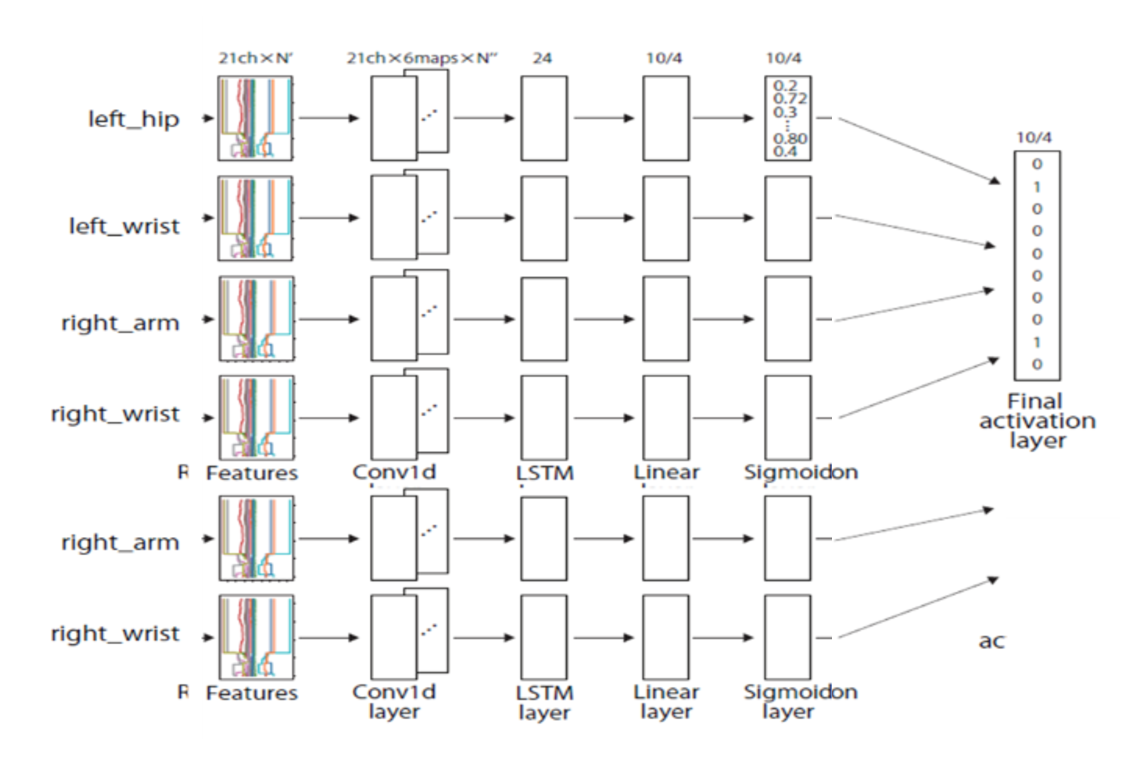
\includegraphics[width=0.9\linewidth]{figures/model.eps}
    \caption{Details of our model. The first layer is preprocessed 21-dimensional features. Conv1d layer is one dimensional convolutional layer. This layer accepts 21-dimensional time-series features and maps each dimension to six (i.e. 21-dimensional features $\times$ 6 maps $=$ 126-channel). The LSTM layer consists of 24 hidden layer, accepts 126-channel time-series data, and outputs 24-dimensional tensors. The linear layer transforms 24-dimensional tensors into 10-dimensional ones. After applying the sigmoid function in the sigmoid layer, the six predictions are merged to obtain the final prediction result.}
    \label{fig:model}
\end{figure}

\begin{itemize}
    \item {\bf Conv1d layer} has an input of 21 channels $\times$ sequence length $N$ and an output of 21 channels $\times$ map size $M$ $\times$ sequence length $N'$. $N$ is the length of hand crafted time-series feature data, which is shorter than the raw data. $N'$ is the length of time-series data after the one dimensional convolution. This is equal to $N-K+1$ ($K$ is the kernel size). $N$ and $N'$ varies with the data because the dataset contains missing data. Kernel size $K$ is set to 5. If $N$ is 4, $N'$ will be 0. Therefore, segments with $N$ shorter than 5 are discarded and not fed into the model. Map size $M$ is the number of filters and set to 6 $\times$ 21-dimensional features $=$ 126. There are 6 filters for each channel, and the convolution is conducted for each channel.
    
    \item {\bf LSTM layer} has an input of 126 channels $\times$ sequence length $N'$ and an output of 24-dimensional tensors. This LSTM solves the many to one task. We set the number of hidden layers to 24. The outputs obtained from the LSTM are not time-series data, but simply tensor.
    
    \item {\bf Linear layer} has an input of 24-dimensional tensor and an output of 10-dimensional tensor which is the same as the number of activity classes.
    
    \item {\bf Sigmoid layer} applies the sigmoid activation function to the 10-dimensional tensor. The output 10-dimensional tensor indicates the likelihood that the class is correct. This layer is not used in the training phase.
\end{itemize}



\subsection{Loss Function and Optimizer}
The model is trained on BCEWithLogitsLoss. Since this loss includes a Sigmoid layer, a Sigmoid layer in our model described in Section \ref{subsec:model} is not applied in the training phase. The weight was set to one for all classes. Adam was used for optimizer.



\subsection{Final Prediction Classes Activation}
Through the above process, the predictions for 6 sensors with 10 labels of sigmoid values are obtained. Their labels are shown in Table \ref{tab:activity}. 6 sensors are Right Shoulder, Right Elbow, Right Wrist, Left Shoulder, Left Elbow and Left Wrist. Finally, our method integrates these predictions and outputs the final prediction.
Specifically, the sigmoid values for each class are summed and the final prediction is made. If the total values are the same, the class that contains the largest value among each label is adopted.

For example, if the predicted values for activity 1 are [1.0, 0.0, 0.0, 0.0, 0.0, 0.0, 0.0, 0.0, 0.0, 0.0], [0.0, 0.5, 0.0, 0.0, 0.0, 0.0, 0.0, 0.0, 0.0, 0.0], [0.0, 0.5, 0.0, 0.0, 0.0, 0.0, 0.0, 0.0, 0.0, 0.0], [0.0, 0.0, 0.5, 0.0, 0.0, 0.0, 0.0, 0.0, 0.0, 0.0], [0.0, 0.0, 0.0, 0.0, 0.0, 0.0, 0.3, 0.0, 0.1, 0.0], [0.0, 0.0, 0.0, 0.0, 0.0, 0.0, 0.0, 0.0, 0.5, 0.0].
The summed sigmoid values are [1.0, 1.0, 0.5, 0.0, 0.0, 0.0, 0.3, 0.0, 0.6, 0.0], and the label with the largest value is adopted. However, in this case, the maximum value of 1 exists in label 1 and label 2, therefore we go back to the predicted values in each sensor. In the original prediction, the maximum value in label 1 is 1 and the maximum value in label 2 is 0.5, therefore we adopt label 1.

%以上の過程を経て,10クラスのシグモイド値を持つ6つのセンサの予測値が得られる.そして,これらの予測値を統合し,最終的な予測値を出力します

%具体的には,各クラスのシグモイド値を合計し,最終的な予測を行います.合計値が同じであれば,各クラスの中で最も大きな値を含むクラスが採用される。

%例えば、アクティビティ1の予測値が[1,0,0,0,0,0,0,0]、[0,0.5,0,0,0,0]、[0,0.5,0,0,0,0,0,0]、[0,0. 5,0,0,0,0,0]、[0,0,0.5,0,0,0,0,0]、[0,0,0,0,0,0,0,0,0,0]の場合。シグモイドの合計値は[1,1,0.5,0,0,0,0,0,0,0,0,0,0]となり、最大値を持つクラスが採用されます。しかし,今回の場合,クラス1とクラス2に最大値1が存在するため,各センサの予測値に戻ります.元の予測値では,クラス1の最大値は1,クラス2の最大値は0.5なので,今回はクラス1を採用します.



% 4
\section{Implementation}
\label{sec:implementation}
In partitioning process, repetitions were identified by calculating autocorrelation using \texttt{tsa.stattools.acf}\footnote{\url{https://www.statsmodels.org/stable/generated/statsmodels.tsa.stattools.acf.html}} in \texttt{statsmodels} library. The model is developed in PyTorch. The loss function and optimizer was implemented using PyTorch libraries\footnote{\url{https://pytorch.org/docs/stable/generated/torch.nn.BCEWithLogitsLoss.html}}\footnote{\url{https://pytorch.org/docs/stable/generated/torch.optim.Adam.html}}.



% 5
\section{Evaluation}
\label{sec:evaluation}
This section describes the evaluation environment. In the training phase, all data of train subjects were used for training in one epoch, which was iterated 5,000 epochs. Table \ref{tab:result} shows accuracy and loss for the six sensor positions at 5,000 epochs by changing training and testing subjects. The loss was calculated using the 10-dimensional tensor output from the linear layer described in Section \ref{subsec:model}.

\begin{table}[h]
    \centering
    \caption{Accuracy and loss for the six sensor positions at 5,000 epochs by changing training and testing subjects.}
    \label{tab:result}
    \begin{tabular}{c|c|c|c|c}\hline\hline
    Training data & Test data & Sensor position & Accuracy & Loss \\ \hline
    \multirow{6}{*}{Subject 1, 2} & \multirow{6}{*}{Subject 3} & Right Shoulder & 0.135 & 0.238 \\
    & & Right Elbow & 0.137 & 0.266 \\
    & & Right Wrist & 0.127 & 0.272 \\
    & & Left Shoulder & 0.118 & 0.265 \\
    & & Left Elbow & 0.119 & 0.261 \\
    & & Left Wrist & 0.136 & 0.270 \\ \cline{1-5}
    \multirow{6}{*}{Subject 1, 3} & \multirow{6}{*}{Subject 2} & Right Shoulder & 0.136 & 0.250 \\
    & & Right Elbow & 0.121 & 0.290 \\
    & & Right Wrist & 0.133 & 0.284 \\
    & & Left Shoulder & 0.097 & 0.280 \\
    & & Left Elbow & 0.092 & 0.282 \\
    & & Left Wrist & 0.134 & 0.279 \\ \cline{1-5}
    \multirow{6}{*}{Subject 2, 3} & \multirow{6}{*}{Subject 1} & Right Shoulder & 0.142 & 0.236 \\
    & & Right Elbow & 0.130 & 0.276 \\
    & & Right Wrist & 0.115 & 0.282 \\
    & & Left Shoulder & 0.110 & 0.278 \\
    & & Left Elbow & 0.127 & 0.267 \\
    & & Left Wrist & 0.110 & 0.280 \\ \hline
    \end{tabular}
\end{table}

From these results, average accuracy of 0.123 was achieved among subjects 1, 2, and 3 in leave-one-subject-out manner. Even if we take into account the fact that there are 10 classes of labels, this accuracy is not high. The reason for the low accuracy could be that some sensor data was missing or mislabeled. Comparing the results using test data of subject 1, 2 and 3, there does not seem to be a significant difference in accuracy. However, the accuracy of the sensor on the right side of the body tended to be higher than that of the sensor on the left side. This may be due to the fact that subjects are right-handed and the noise in the right half of the body motion is reduced.\par
Note that for submitted result for the data of subject 4, our model was trained separately for the body parts with the data of subjects 1, 2, and 3, and the model at 5,000th epoch was used for testing the data of subject 4.



% 6
\section{Conclusion}
\label{sec:conclusion}
This paper reported the solution of our team ``RitsBen'' to Bento Packaging Activity Recognition Challenge. Our approach leverages autocorrelation function, convolution layer, and LSTM to recognize activities. The evaluation results showed that average accuracy of 0.123 were achieved among subjects 1, 2, and 3 in leave-one-subject-out manner. %We plan to search for parameters and body parts that will further improve the accuracy.



\bibliographystyle{spmpsci}
\bibliography{references}



\section*{Appendix}
\addcontentsline{toc}{section}{Appendix}

\begin{table}[h]
    \centering
    \caption{Our resources.}
    \begin{tabular}{c|l}\hline
    \multirow{6}{*}{Used sensor modalities} & Right Shoulder \\
    & Right Elbow \\
    & Right Wrist \\
    & Left Shoulder \\
    & Left Elbow \\
    & Left Wrist \\ \hline
    \multirow{7}{*}{Features used} & Mean \\
    & Variance \\
    & Max \\
    & Min \\
    & Root mean square \\
    & Interquartile range \\
    & Zero crossing rate \\ \hline
    \multirow{3}{*}{Programming language and libraries used} & Python 3.8.8 \\
    & statsmodels 0.12.2 \\
    & PyTorch 1.9.0 \\ \hline
    \multirow{2}{*}{Window size and post processing} & Window size: 400 ms \\
    & Overlap: 50 ms \\ \hline
    \multirow{2}{*}{Using resources in training and testing} & CPU memory: 3043MB \\
    & GPU memory: 271MB \\ \hline
    \multirow{2}{*}{Training and testing time} & Training time (during 5,000 epoch): 1112.233 sec \\
    & Testing time (at 5,000 epoch): 5.577 sec \\ \hline
    \multirow{4}{*}{Machine specification} & OS: Windows 10 Pro \\
    & CPU: Intel Core i9-10900K 3.70GHz \\
    & RAM: DDR4 128GB \\
    & GPU: NVIDIA GeForce RTX 3060 GDDR6 12GB \\ \hline
    \end{tabular}
\end{table}

% \subsection*{Used sensor modalities}
% Six sensors at right shoulder, right elbow, right wrist, left shoulder, left elbow, and left wrist from three subjects were used.


% \subsection*{Features used}
% Seven kinds of features were used: Mean, variance, max, min, root mean square (RMS), interquartile range (IQR), and zero crossing rate (ZCR). These features are extracted for x, y, and z axis, respectively.


% \subsection*{Programming language and libraries used}
% Python 3.8.8 was used. For network implementation, PyTorch 1.9.0 was used.


% \subsection*{Window size and post processing}
% Window size of 400 msec and an overlap of 50 msec.


% \subsection*{Training and testing time}
% Training and testing time (5,000 epoch) was 21.554s and 28.891s.


% \subsection*{Machine specification}
% OS: Windows 10 Pro. CPU: Intel Core i9-10900K 3.70GHz. RAM: DDR4 128GB. GPU: NVIDIA GeForce RTX 3060 GDDR6 12GB.





\end{document}
